\iffalse 

TODO : 
参考文献修正、フッターに書く?
リストのマークを変える、サイズ大きく
本文文字太くする?
画像があるといい

\fi

\RequirePackage{plautopatch} 
\documentclass[17pt,aspectratio=169]{beamer} 
\usepackage{amsmath}
\usepackage{graphicx}
\usepackage{luatexja}
\usepackage{luatexja-fontspec} 
\usepackage{fontspec}
\usepackage{color}
\usepackage{tcolorbox}
\usepackage{ascmac}
\usepackage{bm}

\usepackage{enumitem}
\setlist[itemize,1]{label=\textbullet, itemsep=17pt}  % 記号をもうちょっと大きくしたい
\setlist[itemize,2]{label=\textasteriskcentered, itemsep=3pt} 

\usetheme{metropolis}  % Metropolisテーマを使用
\setmainjfont{Yu Gothic Bold}  
\setsansjfont{Yu Gothic Bold}  

%Beamerフォント設定
\usefonttheme{professionalfonts} % Be professional!
\usepackage[T1]{fontenc}
\usepackage{mlmodern}  % 太いComputer Modern
% MLmodernのバグを修正: cf. https://tex.stackexchange.com/questions/646333/size-of-integral-symbol-in-section-header-with-mlmodern
\DeclareFontFamily{OMX}{mlmex}{}
\DeclareFontShape{OMX}{mlmex}{m}{n}{%
   <->mlmex10%
   }{} 
\renewcommand{\familydefault}{\sfdefault}  % 英文をサンセリフ体に
\renewcommand{\kanjifamilydefault}{\gtdefault}  % 日本語をゴシック体に
\usefonttheme{structurebold} % タイトル部を太字
\setbeamerfont{alerted text}{series=\bfseries} % Alertを太字
\setbeamerfont{section in toc}{series=\mdseries} % 目次は太字にしない
\setbeamerfont{frametitle}{size=\large} % フレームタイトル文字サイズ
\setbeamerfont{title}{size=\LARGE} % タイトル文字サイズ
\setbeamerfont{date}{size=\small}  % 日付文字サイズ
\setbeamerfont{normal text}{series=\mdseries} % 本文を太字に 

%ページ番号の設定
\setbeamertemplate{footline}{
    \hfill {\textcolor{gray!90}{\insertframenumber/\inserttotalframenumber}\hspace{0.1cm}}
    \vspace{0.1cm} 
}

%短縮形
\newcommand{\Pbb}{\mathbb{P}}
\newcommand{\Gcal}{\mathcal{G}}
\newcommand{\Fcal}{\mathcal{F}}

%タイトル
\title{¬ACの相対的無矛盾性のIsabelle/ZFによる形式的証明}
\author{東北大学情報科学研究科 住井・松田研究室 \\ 舟根大喜}
\date{\today}

\begin{document}
\maketitle

\begin{frame} {参考文献}
    \begin{itemize}
        \item Kenneth Kunen著, 藤田 博司 訳 (2008) \\「集合論: 独立性証明への案内」
        \item Thomas Jech著 (2008) 「the Axiom of Choice」
        \item Thomas Jech著 (2002) 「Set Theory」
        \item Asaf Karagila著 (2023) \\ 「Lecture Notes: Forcing \& Symmetric Extensions」 \\
              {\small (https://karagila.org/files/Forcing-2023.pdf) }
    \end{itemize}
\end{frame}

\section{Isabelle/ZFについて}

\begin{frame}{定理証明支援系}
    \begin{itemize}
        \item 数学的証明の形式化や、\\ソフトウェアの正しさの証明\\などに用いられるシステム
        \item プログラムを書くように定義・証明を記述する
    \end{itemize}

    %定理証明支援系のイメージ画像

\end{frame}

\begin{frame}{Isabelle}
    \begin{itemize}
        \item 定理証明支援系の一つ
        \item 初版は1986年
              {\small \begin{itemize}
                  \item Lawrence Paulsonらによる
              \end{itemize} }
        \item 現在も開発・利用が続けられている
    \end{itemize}

    %Isabelleのロゴ画像 Isabelle2024?
    %https://isabelle.in.tum.de/index.html Isabelleの公式サイト 
    %archiveの画像

\end{frame}

%----------------------------------------------
%    Isabelleの実績: seL4マイクロカーネルの正式な仕様と証明
%    https://read.seas.harvard.edu/~kohler/class/cs260r-17/klein10sel4.pdf
%----------------------------------------------

%Pureの説明or画像があるといいかも

\begin{frame}{Isabelle}
    \begin{itemize}
        \item 論理体系「Pure」上で定理証明を行う
        \item 「Pure」上に他の論理体系が構築されている
              {\small \begin{itemize}
                  \item Heigher-Order Logic
                  \item First-Order Logic \\
                  \item \dots
              \end{itemize} }
    \end{itemize}
    \vspace{-10pt}
\end{frame}

% 簡単な定理証明の例を紹介するといいかも
% apply-script, structured proofの説明

\begin{frame}{Isabelle/ZF}
    \begin{itemize}
        \item Isabelle上で一階述語論理とZF(C)公理系を\\用いて証明を行うためのフレームワーク
    \end{itemize}
\end{frame}

% ZFの公理を記述しているコードを紹介するといいかも
% https://isabelle.in.tum.de/dist/library/FOL/ZF/ZF_Base.html ZFの公理のコード


\section{集合論の形式化に関する\\先行研究 }

\begin{frame}{先行研究 (Isabelle/ZF)}

    %----------------------------------------------
    %    IsabelleとLeanで先行研究がある
    %    Isabelle/HOL上でZF集合論をやる研究もある
    %----------------------------------------------

    \begin{itemize}
        \vspace{10pt}

        \item \textbf{構成可能集合の形式化}
              {\small \begin{itemize}
                      \item Lawrence C. Paulson(2002)
                      \item ACがZF上相対的無矛盾であることの証明
                  \end{itemize} }
              % https://www.cl.cam.ac.uk/techreports/UCAM-CL-TR-551.pdf 論文リンク

        \item 強制法の形式化 \& CHのZFC上の独立性証明
              {\small \begin{itemize}
                  \item Emmanuel Guntherら(2020,2022)
                  \item Kunenの強制法の章を形式化
                  \item c.t.m.の存在を仮定しその上のpreorderを用いる
              \end{itemize} }

              % https://arxiv.org/pdf/2001.09715 強制法の形式化
              % https://cs.famaf.unc.edu.ar/~pedro/forcing/Independence_CH/document.pdf CHの独立性証明
    \end{itemize}
\end{frame}

\begin{frame}{先行研究 (Lean)}
    \vspace{10pt}

    \begin{itemize}
        \item 強制法の形式化 \& CHのZFC上の独立性証明
              {\small \begin{itemize}
                  \item Jesse Michael Han, Floris van Doorn(2020)
                  \item flypitchプロジェクト
                  \item ブール値モデルを用いた証明
              \end{itemize} }

        \item QuineのNFのZFC上の相対的無矛盾性証明
              {\small \begin{itemize}
                  \item Sky Wilshaw(2024)
              \end{itemize} }

              %----------------------------------------------
              % https://leanprover-community.github.io/con-nf// 
              % Leanの型理論は(ZFC+可算個の到達不能基数の存在)上無矛盾
              % 到達不能基数の方の仮定は証明でいらないのでZFC上でいいらしい  
              %----------------------------------------------
    \end{itemize}
\end{frame}

\section{本研究}

\begin{frame}{本研究}
    \begin{itembox}[l]{やったこと}
        \begin{center}
            $\neg$ACがZF上相対的無矛盾であることを\\Isabelle/ZFで証明
        \end{center}
    \end{itembox}

    背景
    \vspace{-10pt}
    {\small
        \begin{itemize}
            \setlength{\itemsep}{1pt}
            \item コーエンはCHとACがZFから独立であることを示した
            \item CHの独立性は形式化されている
            \item ACも形式化したい
        \end{itemize}

        %----------------------------------------------
        % ただし、コーエンの証明そのままを形式化したわけではない
        %----------------------------------------------
    }
\end{frame}

\begin{frame}{本研究のアプローチ}
    \vspace{10pt}

    \begin{itemize}
        \item Isabelle/ZFを用いる
              {\small \begin{itemize}
                  \item ZFに関する定義・補題・糖衣構文が多い

                        %----------------------------------------------
                        % Leanの強制法の形式化はLean3でやっている
                        % 最新はLean4で、Lean3と完全に互換性あるわけではない
                        % Lean4に引き継げるのかよくわからなかった
                        %----------------------------------------------

              \end{itemize}}
        \item 証明の基本方針はAsaf Karagilaの講義ノート
              {\small \begin{itemize}
                  \item Lecture Notes: Forcing \& Symmetric Extensions (2023)
                  \item c.t.m.とpreorderを用いた証明
                  \item すでにある強制法の形式化と相性が良い
              \end{itemize} }

              %講義ノートの写真・リンクいる?
              %The axiom of choiceも参考にしていることを書く?
    \end{itemize}
\end{frame}

\section{証明概略}
\begin{frame}{証明概略}
    ZFのc.t.m.$M$から出発し、ZF+$\neg$ACのモデルを構成
    \begin{itemize}
        \item あるposet $\mathbb{P}$によるgeneric拡大$M[G]$について\\
              \textcolor{red}{symmetric extension}と呼ばれる\\
              部分モデル$N \subseteq M[G]$を構成
        \item $N$はZFを満たすが、整列可能定理を満たさない
    \end{itemize}
\end{frame}

\begin{frame}{symmetric extensionの定義(1)}
    \begin{itembox}[l]{定義 (自己同型)}
        {\small
            $(\Pbb, \le_{\Pbb})$は半順序で、最大元$1_{\Pbb}$をもつとする \\
            $\pi : \Pbb \rightarrow \Pbb$が自己同型であるとは次を満たすこと
            \begin{itemize}
                \setlength{\itemsep}{3pt}
                \item $\pi$は全単射
                \item $p, q \in \Pbb$に対して、$p \le_{\Pbb} q \Leftrightarrow \pi p \le_{\Pbb} \pi q$
            \end{itemize}
            $\pi$は以下のように$M^\Pbb$上の自己同型に拡張される
            $$ \pi \dot{x} = \{ (\pi \dot{y}, \pi p) | (\dot{y}, p) \in \dot{x} \} $$
        }
    \end{itembox}
\end{frame}


\begin{frame}{symmetric extensionの定義(2)}
    \begin{itembox}[l]{定義(normal filter)}
        {\small
            $\Gcal$を$\Pbb$の自己同型群とする \\
            $\Gcal$の部分群の族$\Fcal$がnormal filterであるとは次を満たすこと
            \begin{itemize}
                \setlength{\itemsep}{3pt}
                \item $H_1, H_2 \in \Fcal$に対して$H_1 \cap H_2 \in \Fcal$
                \item super groupをとる操作で閉じている
                \item $H \in \Fcal, \pi \in \Gcal$に対して$\pi H \pi^{-1} \in \Fcal$
            \end{itemize} }
    \end{itembox}
\end{frame}

\begin{frame}{symmetric extensionの定義(3)}
    \begin{itembox}[l]{定義 (hereditarily symmetric)}
        {\small
            $\Fcal$を$\Gcal$のnormal filterとする
            \vspace{5pt}
            \begin{itemize}
                \setlength{\itemsep}{2pt}
                \vspace{-10pt}
                \item $\dot{x} \in M^\Pbb$が$\Fcal$-symmetric $\Leftrightarrow \{ \pi \in \Gcal | \pi \dot{x} = \dot{x} \} \in \Fcal$
                \item $\dot{x}$がhereditarily $\Fcal$-symmetricとは以下を満たすこと
                      \vspace{-3pt}
                      \begin{itemize}
                          \item $\dot{x}$は$\Fcal$-symmetric
                          \item $\bm{\mathbf{dom}}(\dot{x})$の全ての要素はhereditarily $\Fcal$-symmetric
                      \end{itemize}
                \item hereditarily $\Fcal$-symmetricな$\dot{x}$の集合を$\bm{\mathbf{HS}}_{\Fcal}$とかく
                      %\item $\Pbb$-generic filter $G$に対し、\\$N = \{ \dot{x}_G | \dot{x} \in \bm{\mathbf{HS}}_{\Fcal} \}$をsymmetric extensionという
            \end{itemize}
        }
    \end{itembox}
\end{frame}

\begin{frame}{symmetric extensionの定義(4)}
    \begin{itembox}[l]{定義 (symmetric extension)}
        {\small
            $\Pbb$-generic filter $G$に対し、\\$\{ \dot{x}_G | \dot{x} \in \bm{\mathbf{HS}}_{\Fcal} \}$をsymmetric extensionという
        }
    \end{itembox}
\end{frame}

\section {Isabelle/ZFによる形式化}

\begin{frame}{成果}
    本研究で証明した主定理
    \vspace{-1cm}
    \hspace{-1.5cm}
    \begin{figure}
        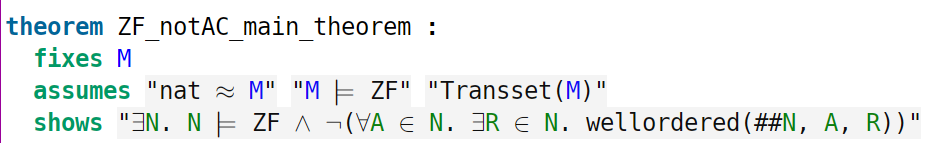
\includegraphics[width=1.1\linewidth]{./images/ZF_notAC_main_theorem.png}
    \end{figure}

    \vspace{-5pt}
    意味 \\
    {\small
    \hspace{1cm} $M$をZFのc.t.m.とする。このとき、ある$N$があって、\\
    \hspace{1cm} $N$はZFを満たすが、整列可能定理を満たさない
    }
\end{frame}

\begin{frame}{作業工程}
    以下の工程に分けられる
    \begin{itemize}[itemsep=8pt]
        \item symmetric extensionの定義
        \item ZFのモデルであることの証明
        \item 特定のsymmetric extensionの構成
        \item それが$\neg$ACを満たすことの証明
    \end{itemize}
\end{frame}

\begin{frame}{作業量}
    \makebox[\textwidth]{約1万5千行のコード \hfill {\small 補題など(3千行)}}
    {\small
        \begin{itemize}[itemsep=8pt]
            \item symmetric extensionの定義(3千行)
            \item ZFのモデルであることの証明(5千行)
            \item 特定のsymmetric extensionの構成(2千行)
            \item それが$\neg$ACを満たすことの証明(2千行)
        \end{itemize} } 
\end{frame}

\begin{frame}{苦労した点(1)}
    「自明なこと」の証明が非常に大変な場合がある \\
    例えば...
    {\small
    \begin{itemize}
        \item 定義した関数が「本当に関数であること」
        \item クラスに対し「本当にそれを表す論理式が存在すること」
    \end{itemize}
    }
\end{frame}

\begin{frame}{苦労した点(2)}
    先行研究の強制関係の定義が少し特殊
\end{frame}

\begin{frame}{苦労した点(3)}
    ZFのモデルであることの証明
\end{frame}

\section {まとめ}

\begin{frame}{まとめ}
\end{frame}

\end{document}


\iffalse
    主定理のコード
    定義を掘っていく

    どのように集合論を表現しているか
    論理式・充足関係

    行程の説明

    全体的に苦労した点
    Mの元であることの証明



\fi